

\chapter{Methods\label{cha:methods}}
Data collection on flights passing through the airspace monitored and controlled by Isavia has been going on for several years now. This data is filtered and stored on company servers for reference and analysis. The statistical analysis for this project was done in Python and used to determine the fleet mix at BIKF, runway occupancy and landing intervals.

\section{Data Collecting and Data Filtering}
More detailed data collection commences on 21 November 2014 with the implementation of the Automatic Dependent Surveillance-Broadcast (ADS-B) system by Isavia. ADS-B was preferred to radar at Keflavik International Airport because of improved signal accuracy~\cite{isavia_wiki}. The ADS-B equipped aircraft through Keflavik Airport are estimated to be around~$90\%$~\cite{isavia-rounardeild_rannsoknir_2018}. The aircraft surveillance data specifications used for measurements are in the Eurocontrol ASTERIX Category 21 standard~\cite{ASTERIX_ADS-B_specs}.
The reading from the position of the ADS-B antenna of the aircraft is used instead of the tail and nose positions. This simplification could result in a few seconds difference. Certain filtering of the ADS-B data is applied before commencing measurements and calculations~\cite{isavia_wiki}: 
\begin{itemize}
    \item All records with no latitude, longitude and/or time data are omitted.
    \item The records are filtered with regards to quality, i.e. filtered with regards to Target Surveillance status, MOPS version, NUC/NIC, NACp, SIL and PIC.
    \item An ADS-B data record within 0.5 second from another is omitted, i.e. if there are less than 0.5 seconds between two successive locations one of the records is omitted.
    \item An algorithm is used to analyse the data and determine if it originates from two different flights (the flight stops for 15 minutes or more after/before taxiing). If so the data for the second flight is omitted
    \item The velocity is calculated from ADS-B location data and ADS-B time data (velocity = distance travelled/time). The ADS-B velocity record is optional in the ASTERIX category 21 standard and is therefore unreliable in measurements. Since the velocity is calculated from measured data, it can exhibit spikes. To get a more realistic velocity curve, a Savitzky-Golay filter is applied to smooth the data.
    \item An aircraft main gear lift-off is considered to be the point where the ADS-B ground bit is removed, i.e. the ADS-B ground bit goes from a value of 1 to a value of 0.
    \item An aircraft touchdown is considered to be the point where the ADS-B ground bit is set, i.e. the ADS-B ground bit goes from a value of 0 to a value of 1.
    \item An aircraft is considered to be stationary when the velocity is below 0.5~knots and to be moving if the velocity is greater than 0.5~knots.
    
\end{itemize}

\fxnote{The ROT measurements have been checked by: comparing them to measurements made by hand.
Who measures and who checks them and how???}

\section{Data Manipulation}
The data was obtained from the database using SQL server and stored as csv files. The manipulations on the data frames were performed using the functionality of Pandas and NumPy data analysis tools and computing packages for Python. A key table containing information about 2300 aircraft models, including ICAO and RECAT-EU wake turbulence categories for each model, was also used as reference. 
The reference table was provided by Eurocontrol. 
The Isavia aircraft data was cross-referenced with the Eurocontrol key table based on ICAO aircraft type labels, the mutual characteristic in both data sets. 
After cross-referencing a RECAT-EU category was assigned to each of the aircraft arriving at BIKF in peak hours. Outliers bellow the 0,003~quartile and above the 0,997~quartile were regarded as anomalies and removed from the data-set, based on AROT values. 
The resulting data frame was used for initial analysis in this project. 
It contained over 11500 arrivals for the time period of almost four years (from 01.01.2015 until 30.11.2018). The data frame contained unique information about the AROT of each aircraft, landing time and runway, along with the ICAO wake category. Consequently the time frame for the analysis was reduced to 13 months (from 04.10.2017 to 30.11 2018) because of the effect of fast-exits on AROT, which is explained in the upcoming section \ref{sssec:runway_usage_arot}


\subsection{Aircraft Traffic Mix\label{ssec:traffic_mix}}
The aircraft traffic mix is one of the components that affect runway capacity as mentioned in Section~\ref{sec:runway_capacity}. Sorting the aircraft fleet arriving at BIKF into ICAO WTC reveals that the majority of flights~(85,4\%) are in the Medium wake category (Figure~\ref{fig:post_fast_exit_mix_pie_v2}) and the rest are mainly in the Heavy category~(14,2\%) with less than one percent Light aircraft. The small portion of Light flights can be explained with the policy of ATM at BIKF to avoid servicing those flights during the morning and afternoon peaks. This distribution of the three categories implies that combining the aircraft into arriving pairs would produce primarily Medium-Medium pairs. This is confirmed by the analysis of the number of arrival pairs in the ICAO categories (Table~\ref{tab:pairs_mix_to_wtc}).\\
When this same fleet is presented using the RECAT categories, the prevailing category is CAT-C (73,7\%), followed by CAT-D (22,1\%). The percentage of each of the remaining categories varies within 2\%. The expectation that this distribution of the RECAT categories would result in primarily in C-C pairs is confirmed later on by the analysis presented in Table~\ref{tab:pairs_mix_to_recat}. \\
The method of of re-categorising the traffic mix is a prerequisite for assembling the RECAT pairs later on and determining the main aircraft categories that will be considered for analysis along with estimating the inter arrival distances characteristic of each pair.
\begin{figure}[h]
    \centering
    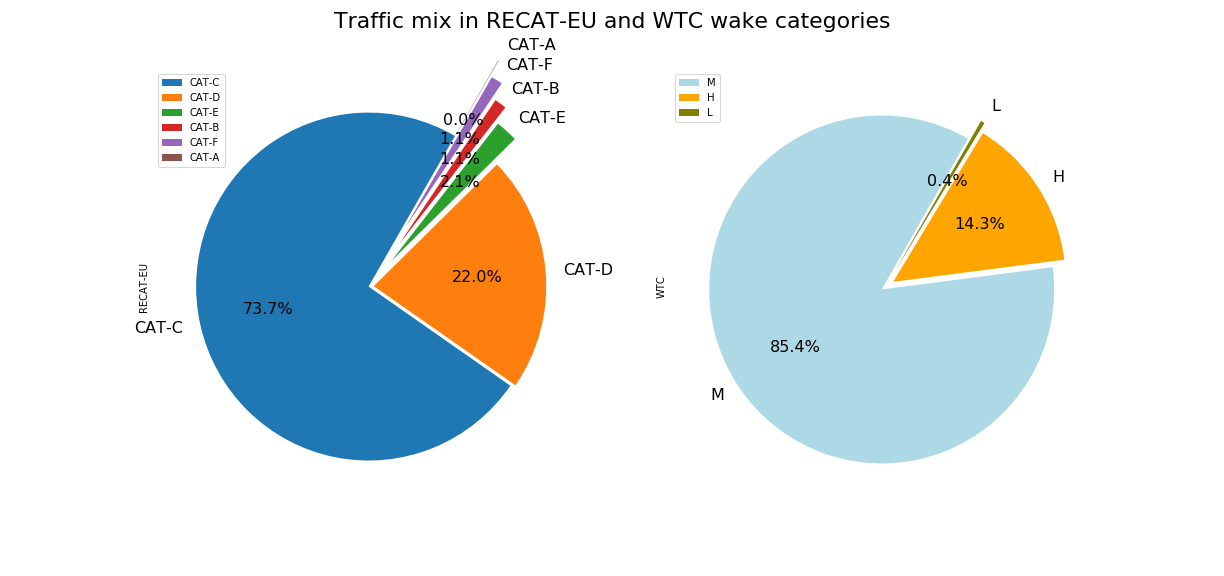
\includegraphics[width=1\textwidth]{graphics/fig_post_fast_exit_mix_pie_v2.png}
    \caption[Traffic mix in RECAT-EU and ICAO WTC]{The traffic mix at Keflavik Airport represented in RECAT-EU categories alongside ICAO WTC categories.}
    \label{fig:post_fast_exit_mix_pie_v2}
\end{figure}
Another approach for classification of the traffic fleet mix at BIKF in peak hours is to identify the aircraft types or models. The traffic data contains ICAO aircraft type designator, that is a two-, three- or four-character code comprising of numbers and letters. This designator is unique for each aircraft type. The top fifteen ICAO types of the aircraft mix are presented in Figure~\ref{fig:traffic_mix_by_model}. Dominating the scene (56.8\% of all arrivals) is the Boeing~757-200 model (ICAO:B752), followed by the Boeing~767-300 (ICAO:B763).
\begin{figure}[h]
    \centering
    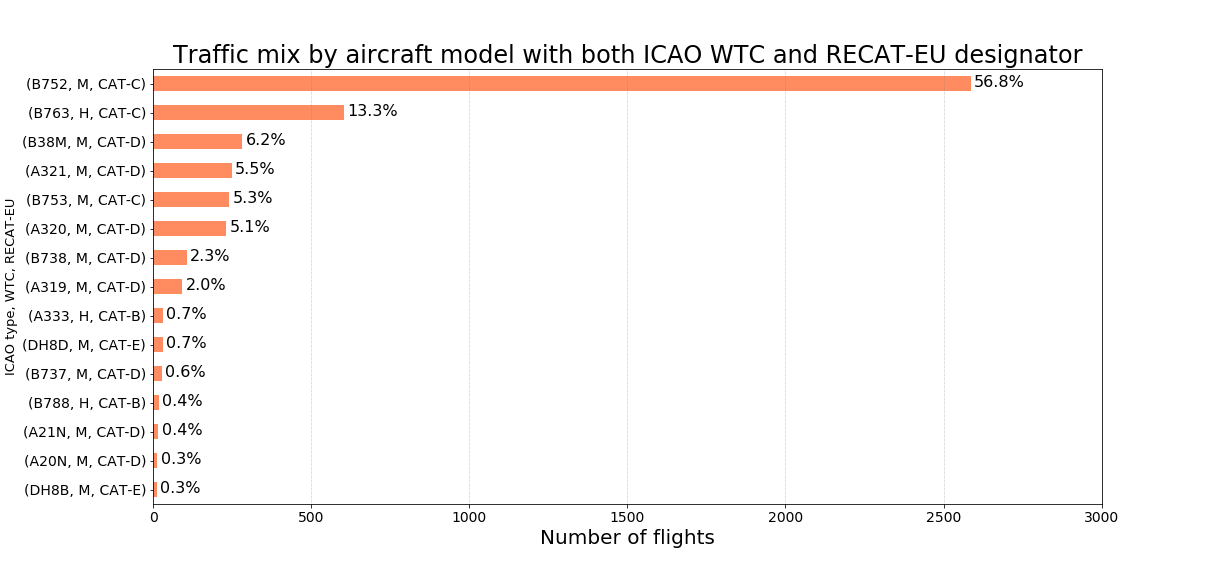
\includegraphics[width=1\textwidth]{graphics/fig_traffic_mix_by_model.png}
    \caption[Traffic mix by aircraft model.]{The traffic mix at Keflavik Airport grouped by aircraft type are shown alongside the ICAO WTC and RECAT-EU designators. The top three models comprise the major part of the Icelandair fleet.}
    \label{fig:traffic_mix_by_model}
\end{figure}
 Those models represent a major part of the Icelandair fleet and the share of the Boeing~737~MAX~8 (ICAO:B38M) is likely to increase as the Icelandair company plans to gradually add sixteen new B38M and B39M models from the beginning of 2018~\cite{icelandair_fleet}. The aircraft types are shown with their ICAO and RECAT categories and the tendency is towards increasing the share of the Medium-Medium pairs, or the C-D and D-C RECAT pairs respectively, with the addition of the new Icelandair aircraft.

% -----------------------

\subsection{Arrival Runway Occupancy Time Considerations}\label{ssec:AROT_considerations} 

The ICAO Doc 4444 PANS-AM~\cite{doc44444} dictates that the radar separation minimum (MRS) between succeeding aircraft which are established on the same final approach track, may be reduced from 3~NM to 2,5~NM under certain conditions. One of the requirements is that the average runway occupancy time of landing aircraft is proven, by means such as data collection and statistical analysis and methods based on theoretical model, not to exceed 50 seconds. 

\subsubsection{Traffic Mix and AROT\label{sssec:mix_effect_arot}}
Several approaches were used to look at the AROT at the airfield. First the runway occupancy was inspected based on the RECAT category of the aircraft (Figure~\ref{fig:RECAT_AROTs_boxplot}). 
\begin{figure}[h]
    \centering
    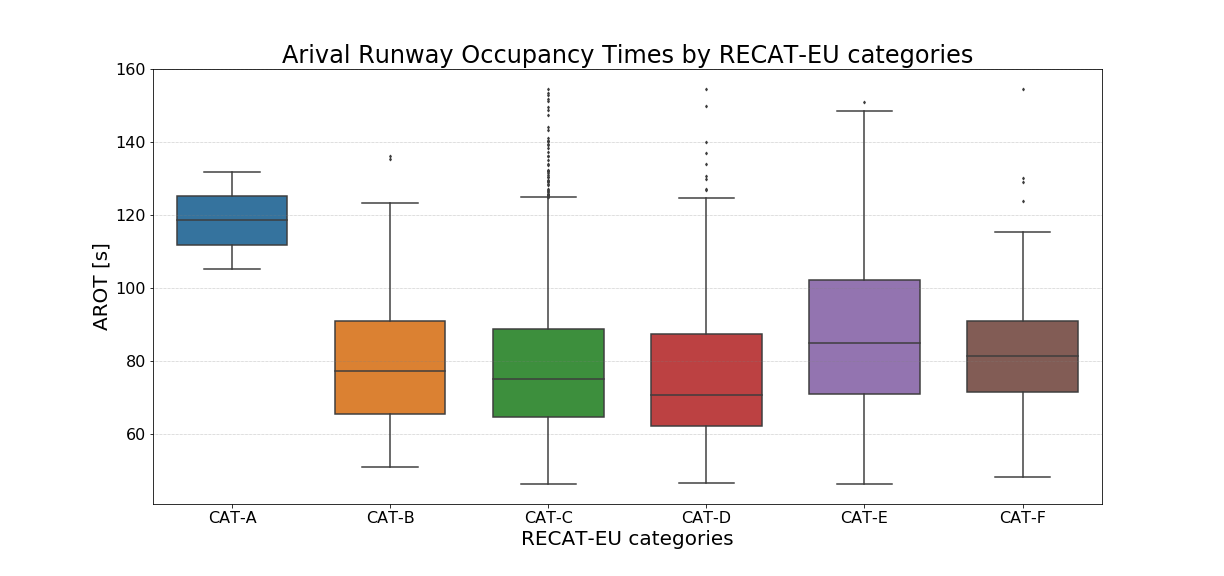
\includegraphics[width=1\textwidth]{graphics/fig_RECAT_AROTs_boxplot.png}
    \caption[AROTs box-plot for RECAT categories, all runways]{Arrival Runway Occupancy Times for the different RECAT-EU categories based on data gathered for a period of one year since October 2017. The coloured blocks indicate where 50\% of the data are or the inter-quartile range (IQR); lower edge is the 25\textsuperscript{th}~percentile, upper edge is the 75\textsuperscript{th}~percentile. The whiskers are at $\pm$1,5$\times$IQR  The box plot shows the AROTs for all runways at BIKF.}
    \label{fig:RECAT_AROTs_boxplot}
\end{figure}
The analysis showed that none of the average runway occupancy values fulfils the 50~seconds limit for reduced MRS. Closest to the required time were the aircraft from the CAT-D and CAT-C with mean values of 75 and 78 seconds respectively (Table~\ref{tab:AROT_RECAT_stats}). Those results point to the necessity of setting the MRS reference value at 3 NM and also suggest that the runway occupancy will be a limiting factor for the cases in which MRS is applicable (Table~\ref{tab:RECAT-dist}). This limitation is also confirmed by the statistical analysis for each of the runways in the following sections.% \ref{sssec:seasonal_arot}, \ref{sssec:runway_usage_arot}. 

\subsubsection{Seasonal Variation of AROT\label{sssec:seasonal_arot}}
Another approach was to analyse the seasonal variations of the runway occupancy. The differentiation between summer and winter months was based on AROT for a period of one year (Table~\ref{tab:month2season_arot}). Months with average AROT~$\leq$80~seconds formed the summer season and the rest were selected as winter months. This separation is purely subjective but succeeds in forming two seasons with equal number of months. On average the seasonal variation of runway occupancy times was eight seconds as seen in Table~\ref{tab:summer_winter_arot}. Sill the seasonal variation should be taken into consideration as they can effect the AROT significantly, especially in the winter months when adverse weather conditions could impair the runway surface by accumulated slush, snow or ice, thus diminishing braking action. Good braking action due to runway surface condition is also one of the requirements for reduced MRS as provided by~\cite{doc44444}.
% Please add the following required packages to your document preamble:
% \usepackage{graphicx}
\begin{table}[h]
\centering
\resizebox{0.8\textwidth}{!} & \multicolumn{1}{l|}{50\%} & \multicolumn{1}{l|}{75\%} & \multicolumn{1}{l|}{max} \\ \hline
\multicolumn{1}{|l|}{SUMMER} & \multicolumn{1}{r|}{3727} & 76  & 17 & 46 & 63  & 72 & 87  & 155 \\ \hline
\multicolumn{1}{|l|}{WINTER} & \multicolumn{1}{r|}{937}  & 84  & 20 & 45 & 69  & 84 & 96  & 153 \\ \hline
\end{tabular}%
}
\caption[AROTs for the air traffic mix by season]{AROT statistics for the air traffic mix at KEF by season. The count is the number of landings in peak hours since October 2017}
\label{tab:summer_winter_arot}
\end{table}

\subsubsection{Runway Usage and AROT\label{sssec:runway_usage_arot}}
Runway occupancy for each of the runways was also examined both with regards to seasonal variations and fast-exit usage. The usage of the four runways in peak hours is shown in Figure~\ref{fig:runway_usage_peak}. 
\begin{figure}[h]
    \centering
    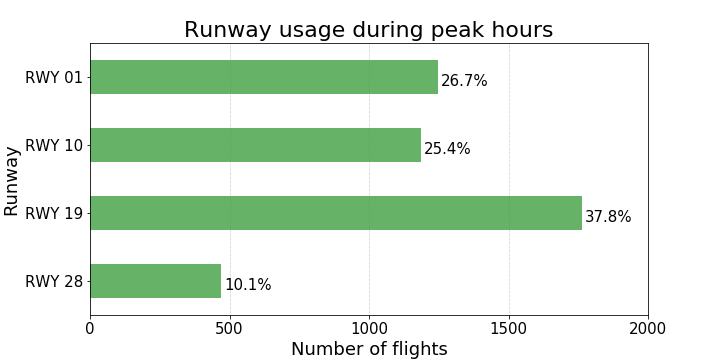
\includegraphics[width=0.8\textwidth]{graphics/fig_runway_usage_peak.png}
    \caption[Runway usage at BIKF during peak hours]{Runway usage at BIKF during peak hours for a period of one year. RWY-19 is the preferred runway, followed by RWY-01 and RWY-10. The RWY-01 is equipped with fast-exit TWY~A-1 and RWY-28 with fast-exit TWY~B-1.}
    \label{fig:runway_usage_peak}
\end{figure}
BIKF airfield is equipped currently with two fast-exit taxiways designated as TWY~A-1 and TWY~B-1. The first was completed on 26~July,~2017 and the later on 4~October,~2017. The date A-1 became operational was chosen as the beginning for the data set considered for analysis in this project. The reason behind this is the beneficial effect that fast-exits have on reducing arrival runway occupancy time. Taxiway A-1 provides a fast-exit track to the left for RWY-01, in the south-north landing direction, and B-1 serves RWY-28 exiting to the right in the east-west direction. The statistical analysis points to decreased AROT on average for RWY-01 after the start of A-1 (Table~\ref{tab:season_AROT_stats_RWY01_pre_fast_exit},~\ref{tab:season_AROT_stats_RWY01_post_fast_exit}). This decrease was primarily during the winter season (12 seconds) but trivial for the summer months. The data for RWY-28 presented a different picture. The average AROT has been reduced by 31 seconds for the summer months and by 37 seconds for the winter, after the implementation of the fast exit (Table~\ref{tab:season_AROT_stats_RWY28_pre_fast_exit},~\ref{tab:season_AROT_stats_RWY28_post_fast_exit}). The minor gain of RWY~01 with TWY~A-1 can be explained with its layout and the fact that A-1 exits into TWY~E-3, meeting taxiing aircraft in the opposite direction (Figure~\ref{fig:BIKF_schematic}), so the fast-exit was avoided altogether in peak hours.\\
% Please add the following required packages to your document preamble:
% \usepackage{graphicx}
\begin{table}[]
\centering
\resizebox{0.8\textwidth}{!} & \multicolumn{1}{l|}{50\%} & \multicolumn{1}{l|}{75\%} & \multicolumn{1}{l|}{max} \\ \hline
\multicolumn{1}{|l|}{RWY 01} & 1247 & 86 & 23 & 46 & 66 & 88 & 101 & 153 \\ \hline
\multicolumn{1}{|l|}{RWY 10} & 1185 & 87 & 12 & 61 & 79 & 86 & 93 & 155 \\ \hline
\multicolumn{1}{|l|}{RWY 19} & 1762 & 68 & 10 & 46 & 62 & 66 & 71 & 155 \\ \hline
\multicolumn{1}{|l|}{RWY 28} & 470 & 69 & 14 & 49 & 61 & 66 & 74 & 155 \\ \hline
\end{tabular}%
}
\caption[AROTs in peak hours by runway]{AROT statistics for the air traffic mix at BIKF in peak hours by runway. The count is the number of landings in peak hours.}
\label{tab:all_RWY_AROT_stats}
\end{table}
Despite the reduced AROT, RWY~28 remained the least used runway, servicing only 10,1$\%$ share of landing aircraft (Figure~\ref{fig:runway_usage_peak}). The preferred runway was RWY~19, servicing 37,8$\%$ of the arrivals. A statistical summary for all the runways is shown in Figure~\ref{tab:all_RWY_AROT_stats}. The average AROT for the BIKF airfield amounted to 77,5 seconds.


% ---------------------------
\subsection{Landing Time Interval}\label{ssec:LTI}
The landing time interval (LTI) in this project is also referred to as inter-arrival time. The method used to determine the LTI required to examine the aircraft in pairs - a leader and a follower. The data-set for the analysis contained the ICAO type and WTC for the leader and the follower along with distance separation and time separation between the aircraft in each pair during peak hours. The time frame was identical with the one used in the previous sections. Additionally every leader and follower were re-categorised and assigned RECAT designator.\\
The information for the arrival pairs was fitted into the ICAO WTC scheme in order to recognise the prevailing aircraft pair mix, which is a consequence of the traffic mix discussed previously in \ref{ssec:traffic_mix}. Clearly the majority of arrival pairs were classified as Medium-Medium (M-M) as shown in Table~\ref{tab:pairs_mix_to_wtc}. The other noticeable pairs were variations of the Heavy and the Medium groups (H-H, H-M, M-H). Those four pair types formed the subset of data to be further analysed and split into RECAT categories. The rest of the pairs containing a Light aircraft were discarded as being inconsistent because of their limited number. 
% Please add the following required packages to your document preamble:
% \usepackage{multirow}
% \usepackage{graphicx}
% \usepackage[table,xcdraw]{xcolor}
% If you use beamer only pass "xcolor=table" option, i.e. \documentclass[xcolor=table]{beamer}
\begin{table}[h]
\centering
\resizebox{0.3\textwidth}{!}{%
\begin{tabular}{cc|r|r|r|}
\cline{3-5}
\multicolumn{1}{l}{} & \multicolumn{1}{l|}{} & \multicolumn{3}{c|}{Follower} \\ \cline{3-5} 
\multicolumn{1}{l}{} & \multicolumn{1}{l|}{} & \multicolumn{1}{c|}{H} & \multicolumn{1}{c|}{M} & \multicolumn{1}{c|}{L} \\ \hline
\multicolumn{1}{|c|}{} & H & \cellcolor[HTML]{FFCC67}56 & \cellcolor[HTML]{FE996B}334 & \cellcolor[HTML]{FFFFC7}2 \\ \cline{2-5} 
\multicolumn{1}{|c|}{} & M & \cellcolor[HTML]{FE996B}368 & \cellcolor[HTML]{FD6864}1809 & \cellcolor[HTML]{FFFFC7}7 \\ \cline{2-5} 
\multicolumn{1}{|c|}{\multirow{-3}{*}{\rotatebox[origin=c]{90}{Leader}}} & L & \cellcolor[HTML]{FFFFC7}3 & \cellcolor[HTML]{FFFFC7}9 & \cellcolor[HTML]{FFFFC7}1 \\ \hline
\end{tabular}%
}
\caption[BIKF traffic mix sorted into ICAO WTC]{Number of ICAO pairs from the traffic mix at BIKF arranged into the corresponding wake categories.}
\label{tab:pairs_mix_to_wtc}
\end{table}

The ICAO WTC scheme specifies a distance separation minima as prescribed in  Table~\ref{tab:ICAO_WTC} ~\cite{rooseleer2015recat}. The probability distributions of the distance separations from the selected four pair-types were examined and presented in Figure~\ref{fig:dist_separ_HH_HM_MH_MM_pairs} along with the ICAO reference separation.  \fxnote{Why are some data to the left of the red line???}
\begin{figure}[h]
    \centering
    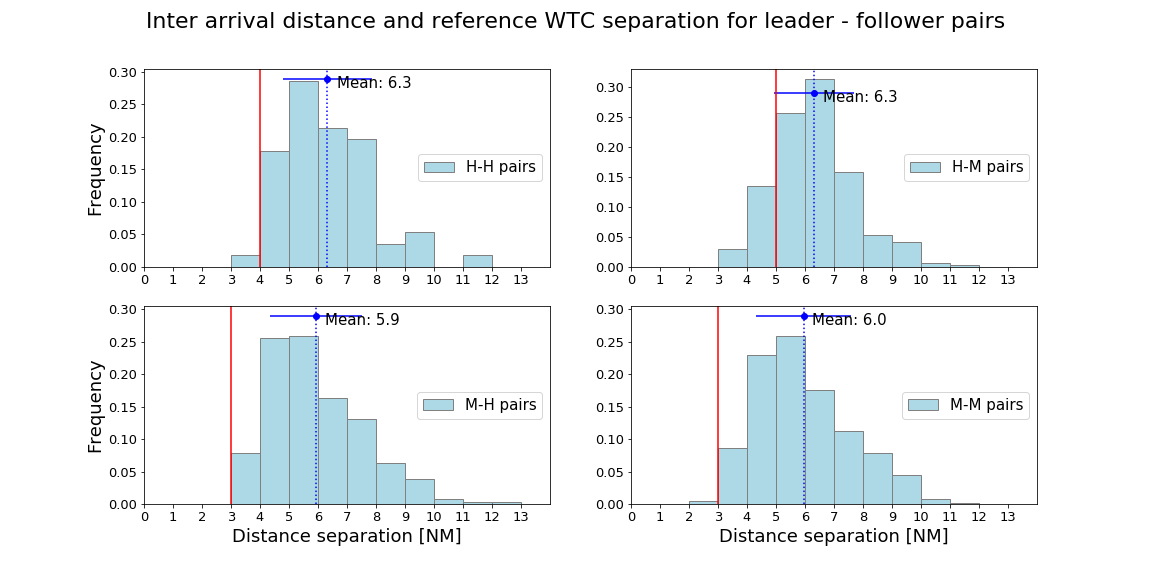
\includegraphics[width=1\textwidth]{graphics/fig_dist_separ_HH_HM_MH_MM_pairs.png}
    \caption[Distribution of distance separation for ICAO pairs]{Distribution of the WTC distance separation between selected ICAO pair categories. The red reference line indicates the separation minima for the particular pair category.}
    \label{fig:dist_separ_HH_HM_MH_MM_pairs}
\end{figure}

Another important metric derived from the data, together with the distance separation between pairs, was the landing time interval, that indicates whether AROT or the separation requirement is a limiting factor for airfield capacity. As stated in the study objective \ref{sec:study_objective} the LTI measures the time separation between aircraft calculated from the distance separation and the final approach speed. This measurement was done for each of the observed pairs and presented in Figure~\ref{fig:time_separ_HH_HM_MH_MM_pairs}, where the reference line indicates the time that a follower takes to travel the distance minima for the respective pair category. The final approach velocity for this calculation was set equal to the maximum average approach velocity from all four runways. This is done by finding the average velocity for each of four runways and using the maximum of the four values as the final approach velocity for the calculation of the LTI. Higher velocity value results in lower time reference. In this sense the reference time is a more liberally specified constraint, as opposed to using the minimum of the approach velocities. Similar methodology is currently being used by Isavia in determining the runway capacity envelope.
\begin{figure}[h]
    \centering
    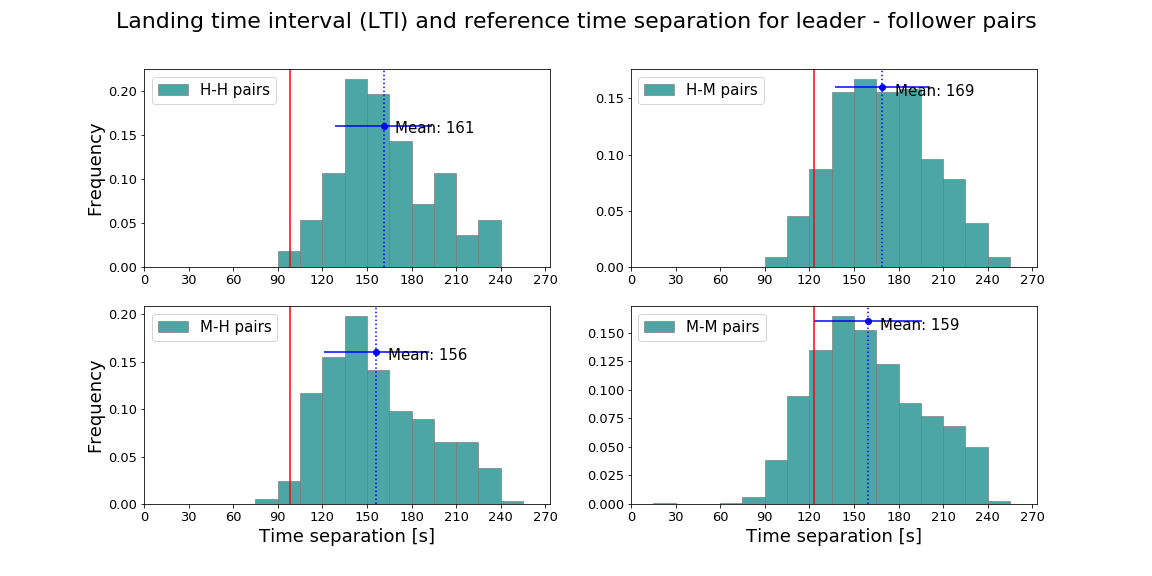
\includegraphics[width=1\textwidth]{graphics/fig_time_separ_HH_HM_MH_MM_pairs.png}
    \caption[Distribution of inter-arrival time separation for ICAO pairs]{Distribution of inter-arrival time separation for selected ICAO pair categories. The red line indicates a liberal time reference estimate for the particular pair category.}
    \label{fig:time_separ_HH_HM_MH_MM_pairs}
\end{figure}














%\lipsum[14-20]
%%% Local Variables: 
%%% mode: latex
%%% TeX-master: "DEGREE-NAME-YEAR"
%%% End: 
